\documentclass[oneside]{book}
\usepackage[utf8]{inputenc}
\usepackage{graphicx}
\usepackage{geometry}
\usepackage{float}
\usepackage{textcomp}
\usepackage{gensymb}
\usepackage{amsmath}
\usepackage{listings}
\geometry{portrait, margin=1. in}
\usepackage[colorlinks = true,
            linkcolor = blue,
            urlcolor  = blue,
            citecolor = blue,
            anchorcolor = blue]{hyperref}

\lstset{language=Python}
\lstset{frame=lines}
%\lstset{caption={Insert code directly in your document}}
%\lstset{label={lst:code_direct}}
\lstset{basicstyle=\footnotesize}



\usepackage{color}

\definecolor{dkgreen}{rgb}{0,0.6,0}
\definecolor{gray}{rgb}{0.5,0.5,0.5}
\definecolor{mauve}{rgb}{0.58,0,0.82}

\lstset{frame=tb,
  language=Java,
  aboveskip=3mm,
  belowskip=3mm,
  showstringspaces=false,
  columns=flexible,
  basicstyle={\small\ttfamily\color{blue}},
  numbers=none,
  numberstyle=\tiny\color{gray},
  keywordstyle=\color{blue},
  commentstyle=\color{dkgreen},
  stringstyle=\color{mauve},
  breaklines=true,
  breakatwhitespace=true,
  tabsize=3,
  %rulecolor=\color{blue},
  %backgroundcolor=\color{darkgray}
}


\begin{document}

\begin{titlepage}
\begin{center}
 {\huge\bfseries SubMIT Off Campus Resources\\}
 % ----------------------------------------------------------------
 \vspace{1.5cm}
 {\Large\bfseries Put Authors Here et. al.}\\[5pt]
 robertej@mit.edu\\
 \href{https://latexonline.cc/compile?git=https\%3A\%2F\%2Fgithub.com\%2Frobertej19\%2FSubMITDocs\&target=main.tex\&command=pdflatex\&trackId=1594872205396}{Live Document Location}\\[14pt]
  % ----------------------------------------------------------------
 \vspace{2cm}


% {By}\\[5pt] {\Large \sc {Me}}
 \vfill
 % ----------------------------------------------------------------

 \vfill
{January 2021}
\end{center}
\end{titlepage}

\tableofcontents

\part{Code Documentation}

    \chapter{Introduction}
        \section{Purpose and General Structure}

The purpose of this software framework is to facilitate the submission of Monte Carlo jobs on GEMC to various computing clusters around the world for CLAS12. The framework uses MySQL databases for information storage and sets of python scripts for running the backend, with a CLAS12 webpage for easy job submission. The general flow is:
\begin{itemize}
  \item User submits an 'scard' (steering card, basically specifications for the simulation)
  \item The scard information is read into the MySQL database, along with user metrics
  \item The scard information is used to generating running scripts 
  \item The running scripts are packaged and submitted to various computing clusters
  \item Computing software frameworks, like HTCondor or Slurm, handle the submission on the cluster
  \item Output is returned to standard CLAS12 output user directories
\end{itemize}


\section{Codebase Structure}
The codebase is almost exclusively written in Python, and is divided as follows:
\begin{itemize}
  \item \textbf{Client} - a client side repository handling the mechanism to get user scard information into a MySQL database
  \item \textbf{Server} - a server side repository handling the mechanism to get job simulation information from MySQL database to computing clusters
  \item \textbf{Utils} - a common repository with organizational scripts for interfacing with user, MySQL database, etc
\end{itemize}
These are the 3 main divisions of the codebase. There are two other important sections:
  \begin{itemize}
    \item \textbf{web interface} This contains all the code for managing the website for the online submission portal
    \item \textbf{Documentation} Documentation for this project. Currently not up to date (\today)+
  \end{itemize}


\section{Documentation and Improvements Needed}
\subsection{Documentation}
The documentation for this project currently needs improvement. It is split across several locations (github, this document, more) and needs to be unified and updated. It is only important for developers (external CLAS12 members do not need to know how this works).
\subsection{Improvement Tasks}
The main areas where this project needs improvement are:
  \begin{itemize}
    \item \textbf{Feature Enhancements} - add more generators, job monitoring, error logging
    \item \textbf{Documentation} - improve the documentation of the project
    \item \textbf{MIT Farms Integration} - give CLAS12 access to MIT's computers through webportal
  \end{itemize}
  
  There are many minor issues that need to be resolved, but the full list of such issues, similar to the documentation, is spread out over several locations and needs to be organized.
        
    \chapter{Client Usage}
        \section{Introduction}
Currently, jobs can be submitted by any CLAS12 member through the online submission portal, or manually by MIT members through either SCOSG16 or SubMIT.
\section{Job Submission through Webportal (Public)}
See \href{https://gemc.jlab.org/web_interface/index.php}{here} and follow instructions
\section{Job Submission through SCOSG16 (Manual)}
Section not yet filled out
\section{Job Submission through SubMIT.mit.edu (Manual)}
\subsection{Description}
The SubMIT system was built to handle job submissions to MIT's Tier 2 (Bates) and Tier 3 (MIT) computing facilities, as well as a few other computing centers around the world. As of 2020, only MIT members have access to submit jobs through this system, but in the end it will need to be opened to all CLAS12 members to submit jobs through the online webportal extension. 
\subsection{Relevant Information}
\href{http://submit.mit.edu/}{SubMIT Information}
\href{http://submit.mit.edu/condormon/index.php}{SubMIT Jobs Monitoring Webpage}
\subsection{Instructions for Manual Job Submission}
Steps for manual job submission, using the user robertej as an example:

        \begin{lstlisting}
            ssh robertej@submit.mit.edu
            cd /work/robertej/jlab_WORKING/clas12simulations
            condor_submit clas12.condor
        \end{lstlisting}
        
        
        Check submitted jobs:
        
        \begin{lstlisting}
            condor_q
        \end{lstlisting}
        

    
    \chapter{Structure}
        


\section{Location of code}
\href{https://gemc.jlab.org/web_interface/index.php}{GEMC web interface}

\href{https://github.com/mit-mc-clas12}{Github Source}

\href{https://gemc.jlab.org/test/web_interface/index.php}{Test GEMC web interface}


%Location of stuff:

 %      inside /group/clas/www/gemc/html/web_interface/stats_results
 %      python /group/clas12/SubMit/utils/jsonify_logfile.py --logfile=gemcRunning.log --output=osgLog.json




\section{DB Schema}
\href{https://dbdiagram.io/d/5c9b829bf7c5bb70c72f6c34}{DB Flowchart (not current)}

update this
All hardcoded information stored in fs.py:

\section{MySQL DB Users}
\begin{center}
\begin{tabular}{ c c c c }
Username & Permissions & Credentials Location & Usage\\
robertej & all & N/A & N/A\\
clas12jrun & read only & msql\_conn.txt & condor\_submit.sh\\
clas12jserver & all & msqlrw.txt & client \& server submit\\
\end{tabular}
\end{center}
        
    \chapter{MIT Computing}
       Send around basic information




        
    \chapter{Developer Usage}
        \section{MySQL Commands}
    For all command examples, we are using the hostname of "jsubmit.jlab.org", the username of "robertej". Substitute these values for your needs. N.b. SQL has a formalism where all commands are capitalized and all items are lower cased. We will try to stick to that in all examples but note that SQL is actually case insenstitive as a language. Also, the language must end each command in a semicolon. \\
    
    
    \subsection{Connecting to Database}
        To establish an interactive session on the command line:
        \begin{lstlisting}
            mysql -h jsubmit.jlab.org -u robertej -p 
        \end{lstlisting}
        
        If you don't want to have an interactive session, or don't want to enter a password each time, you can pass a configuration file as:
        
        \begin{lstlisting}
            mysql --defaults-extra-file=msql_conn.txt     
        \end{lstlisting}
        
        Where mysql\_conn.txt is a text file of the form:
        
        \begin{lstlisting}
            [client]                                                                                            
            user='robertej'                                                                                                   
            password='realpassword'
            host='jsubmit.jlab.org'
            database='CLAS12OCR' 
        \end{lstlisting}
    
    \subsection{Basic MySQL Commands}
    
        See available databases:
        
        \begin{lstlisting}
            SHOW DATABASES;
        \end{lstlisting}
        
        Create a databases:
        
        \begin{lstlisting}
            CREATE DATABASE CLAS12OCR;
        \end{lstlisting}
        
        Delete a databases:
        
        \begin{lstlisting}
            DROP DATABASE CLAS12OCR;
        \end{lstlisting}
        
        Enter a particular database:
        
        \begin{lstlisting}
            USE CLAS12OCR;
        \end{lstlisting}
        
        See available tables in a database:
        
        \begin{lstlisting}
            SHOW TABLES;
        \end{lstlisting}
        
        See schema of a particular table:
        
        \begin{lstlisting}
            DESCRIBE CLAS12OCR.users;
        \end{lstlisting}
        
        Leave the interactive MySQL environment:
        
        \begin{lstlisting}
            EXIT;
        \end{lstlisting}
    
    \subsection{Advanced MySQL Commands}
    
    How to see size of databases (copy verbatim):

        \begin{lstlisting}
            SELECT table_schema "DB Name",
                    ROUND(SUM(data_length + index_length) / 1024 / 1024, 1) "DB Size in MB" 
            FROM information_schema.tables 
            GROUP BY table_schema; 
        \end{lstlisting}
    
    How to dump all information from a database into a text file:
    
    \begin{lstlisting}
        mysqldump -h jsubmit.jlab.org --skip-comments --skip-extended-insert -u robertej -p CLAS12OCR > test10.sql  
    \end{lstlisting}
    
    The two skip options are optional and only include information extraneous to the actual data in the database. They can be omitted without error.\\
    
    How to make a copy of a database to another MySQL DB:

    \begin{lstlisting}
        mysqldump -h jsubmit.jlab.org -u robertej -p CLAS12OCR | mysql -h jsubmit.jlab.org -u robertej -p CLAS12OCRBackup
    \end{lstlisting}    
    
    \subsection{Common MySQL Commands in CLAS12OCR}
    
        Get list of all users and current running jobs:
        
        \begin{lstlisting}
            SELECT user, total_running_jobs FROM users;
        \end{lstlisting}
        
        More usefully, see the 10 most recent submissions on the database:
        
        \begin{lstlisting}
            SELECT user, client_time, run_status FROM submissions ORDER BY user_submission_id DESC LIMIT 10;
        \end{lstlisting}
        
        
        If you want to wrap everything all up in one, you can do: 
        \begin{lstlisting}
        mysql --defaults-extra-file=msql_conn_test.txt -N -s --execute='select user, client_time, run_status from submissions ORDER BY user_submission_id DESC LIMIT 10;' 
        \end{lstlisting}
        
        
        How to copy runscript from the database to a text file:
        \begin{lstlisting}
        mysql --host jsubmit.jlab.org --user='username' --password='password' --database='CLAS12OCR' --execute='SELECT runscript_text FROM Submissions WHERE submissionID = 1; ' > example.txt
        \end{lstlisting}

    \subsection{Permissions in MySQL}
    This section is yet to be populated
    \iffalse
    mysql permissions:
    show users:
    
    select user, host from mysql.db where db='CLAS12OCR';
    
    show grants:
    
    show grants for 'clas12jserver'@'%.jlab.org';
    
    GRANT ALL ON . TO 'clas12jserver'@'%.jlab.org';
    
    current users that access the db:
    
    show processlist;
    
    \fi

\section{Testing with SQLite}
    \subsection*{Create SQLite DB}
        \begin{lstlisting}
            python utils/create_database.py --lite=name.sql
        \end{lstlisting}
    
    \subsection*{Submit job on client side to SQLite DB}
        \begin{lstlisting}
            python client/src/SubMit.py --lite=name.sql -u=username client/scard_type1.txt
        \end{lstlisting}
        
        
         sqlite run to download the running script and the gcard. Assuming DB is in the same dir
    \begin{lstlisting}
        sqlite3 CLAS12_OCRDB.db "SELECT runscript_text FROM
        Submissions WHERE submissionID = $submissionID"  > $nodeScript
    \end{lstlisting}
    
\section{Statistics and Logging}
    \subsection*{GEMC JSON Web Interface Statistics}
         To test on sqlite that things work as intended: 
         \begin{lstlisting}
            python3 utils/gemc_json_logging.py -lite=CLAS12OCR.db -t -o testoutput.log
        \end{lstlisting}
        ~\\
        \newline
        Normal use (with no arguments, default will use mysql db and output to osgLog.json)
        \begin{lstlisting}
            python3 utils/gemc_json_logging.py 
        \end{lstlisting}


\section{Using Travis-CI}
    \href{https://travis-ci.org/}{Travis Location}
    
    Important parts of Travis CI:\\
    There are currently documents important for Travis CI:\\
    
    .travis.yml\\
    requirements.txt\\
    travis.sql\\
    travis\_tests.py\\
    readtests.py\\
    
    \subsection{.travis.yml}
        
        \begin{lstlisting}
        
            language: python
            python:
              - "2.7"
            #  - "3.6"      # current default Python on Travis CI
            # command to install dependencies
            services:
             - mysql
            before_install:
             - mysql -u root --password="" < test/travis.sql
            # - echo "USE mysql;\nUPDATE user SET password=PASSWORD('devpassword') WHERE user='dev';\n" | mysql -u root
            install:
            #  - if [[ $TRAVIS_PYTHON_VERSION == 2.7 ]]; then pip install -r req-py2.txt; fi
            # - pip install -r req-py2.txt; python_version == "2.7"
             - pip install -r test/requirements.txt
            # - pip install mysql-python
            # command to run tests
            
            #script: python2 testapp.py || python3 testapp.py #For now, can't get python3 to work properly
            script: python2 test/travis_tests.py
        \end{lstlisting}
    
    This file must be named as ".travis.yml" and must be found in the main repository directory. It is the launching point for the CI tests. Here you can specify which python versions you want to test, what services to install, and which programs to run.
    
    \subsection{requirements.txt}
        This file contains which python modules need to be installed in the virtual environment. If something is missing, travis will throw an error, so its not so difficult to get right.
        
    \subsection{travis.sql}
                \begin{lstlisting}
                    # Create DB
                    CREATE DATABASE IF NOT EXISTS `CLAS12OCR`;
                    CREATE DATABASE IF NOT EXISTS `CLAS12TEST`;
                \end{lstlisting}
                This initializes the MySQL databases
                
    \subsection{travis\_tests.py}
        This creates all the logically structure and is a framework to execute commands. Its not so important to look at unless something is broken. 
        
    \subsection{readtests.py}
        This is the actual location where what commands to be submitted on Travis-CI are actually specified. The current command structure is:
        
                \begin{lstlisting}
                 verify_submission_success = command_class('Verify scard submission success',
                                    ['sqlite3','utils/CLAS12OCR.db','SELECT user FROM submissions WHERE user_submission_id=1'],
                                    'robertej\n')
                \end{lstlisting}        
        
       The structure is a class where the first element is the desired name of the command (user defined), the second is the actual command to execute on the terminal, broken up between spaces, and the third element is what the expected output is from the command. The default is "0" if no output comparison is desired to be made. Travis will fail if a non-zero output is specified and is not observed, even if the command processes successfully. 
    
    





    


\part{Code Development}   


    \chapter{Resources}
        \section{HTCondor and HTC-Python Bindings}
    \href{http://pages.cs.wisc.edu/~adesmet/status.html}{Status and State Numbers}\\
    \href{https://research.cs.wisc.edu/htcondor/HTCondorWeek2016/presentations/Bockelman_Python-tutorial.pdf}{HTCondor-Python Presentation}\\
    \href{https://research.cs.wisc.edu/htcondor/manual/v8.6/condor_q.html}{Condor\_q Command Documentation}\\
    \href{https://research.cs.wisc.edu/htcondor/mail-lists/}{HTCondor Mailing Lists}\\
    \href{https://htcondor.readthedocs.io/en/latest/apis/python-bindings/index.html}{Python Bindings}\\
    
    
    Even with the above references, some details remained unclear. Here is a useful mapping from python binding commands to condor\_q outputs:\\
    \newline
    \textbf{job.get("ClusterID")} - we have called this different names, but is in the sql db as osg\_ID\\
    \textbf{job.get("JobStatus")} - returns if job is running /idle. See \href{http://pages.cs.wisc.edu/~adesmet/status.html}{Status and State Numbers} for more.\\
    \textbf{job.get("QDate")} - utc unix timestamp of when the job was submitted.\\
    \textbf{job.get("TotalSubmitProcs")} - total number of jobs submitted. To get the number of jobs done, you must subtract all running and idle jobs from the total jobs, i.e. there does not exist a variable tracking how many jobs are done in the batch submission.\\
    
\section{MySQL and SQLite Resources}
    Currently trying to locate these
    
        

    \chapter{Meetings}
        \href{https://bluejeans.com/7572697578}{Meeting Link} \quad \quad
\href{https://latexonline.cc/compile?git=https\%3A\%2F\%2Fgithub.com\%2Frobertej19\%2FSubMITDocs&target=main.tex&command=pdflatex&trackId=1591043936822}{Overleaf Online Location}
\section{Thursday May 28 2020}
    \subsection*{Python Versions}
        \indent We discussed that SubMIT only has python 2.6.6 and has not yet disclosed plans to upgrade / install python3. It was decided to try and write the code to work with python3 as much as possible as it works fine on OSG, SubMIT isn't used much presently, and python2.6 has security flaws.
    \subsection*{Other Notes}
        \indent Mauri and Bobby continue to try to work out python bindings with htcondor.
    





\section{Thursday June 4 2020}
    \subsection*{Using Right Python Path and Modules}
        which python returns /apps/bin/python\\
        need to explicitly use /usr/bin/python2 to get htcondor module to work. I tried changing what "python2" does in bashrc but was getting error messages\\
        /usr/bin/python2 -- this works\\
        /usr/bin/python3 -- no module named 'pytz' (needed for utils/utils.unixtimeconvert()\\
        python2 -- no module named "htcondor"\\
        python3 -- no module named "htcondor"\\

    \subsection*{gemc-jsonify footer issue}
        \begin{figure}[H]
        \centering
        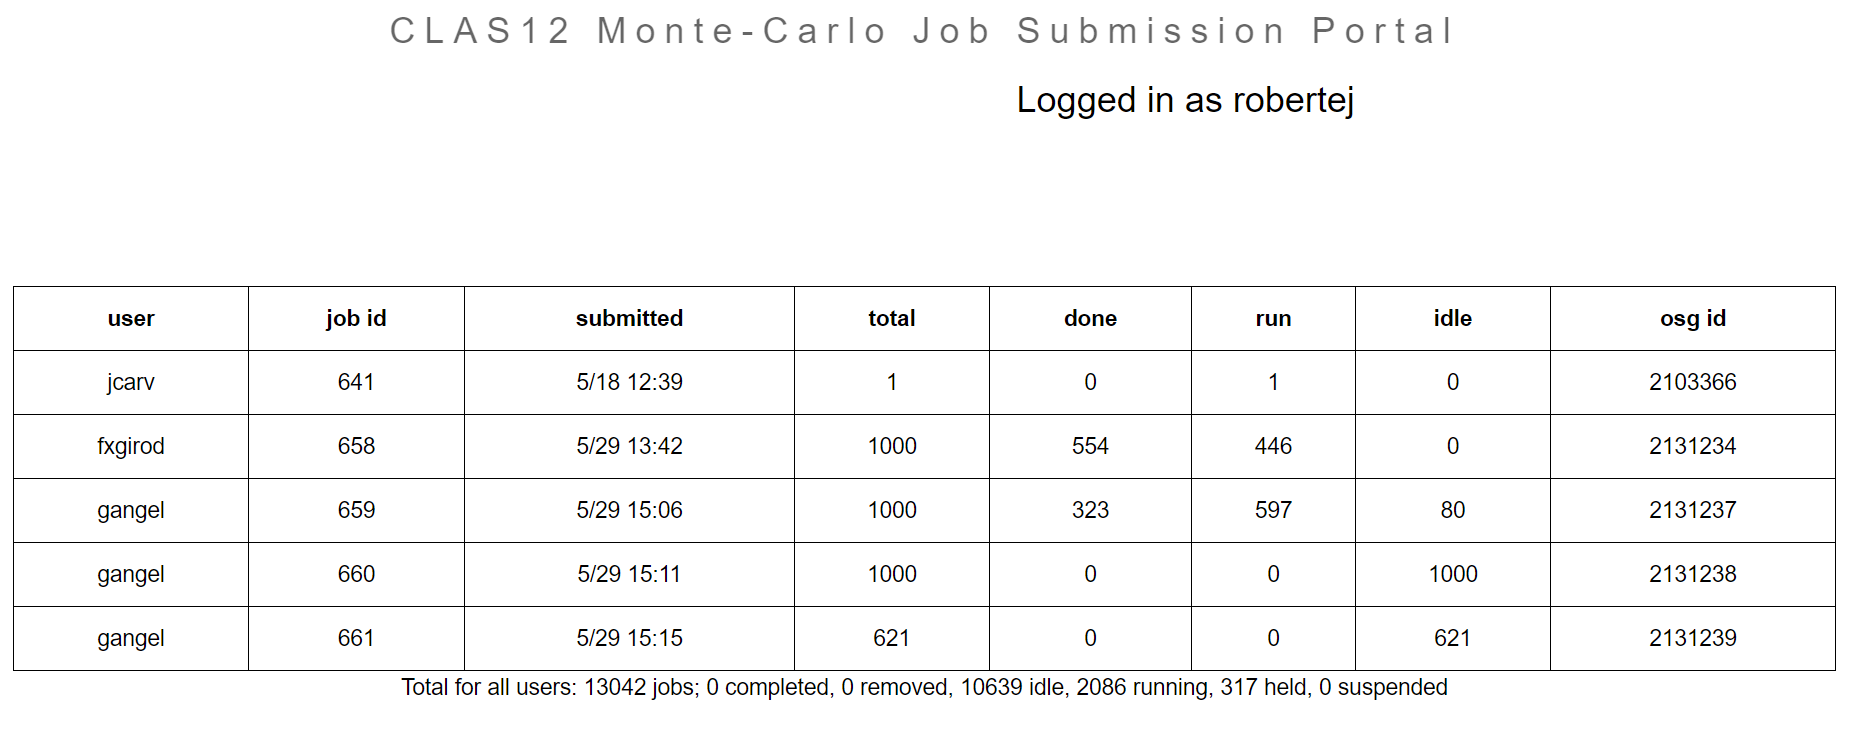
\includegraphics[scale=0.5]{Meetings/20200604/files/jobs-total.PNG}
        \caption{GEMC Web Portal Stats Table Example}
        \label{fig:my_label}
        \end{figure}

    
    Footer metadata - all jobs is for all jobs from JLab, not just CLAS12, this isn't very useful?
    
    \subsection*{Error Handling for when code breaks}
    Error handling: How do we want to handle this? Cant exactly print to screen. Want to send emails when things are breaking? Write to log? something else?
           
    
    \subsection*{Other}
    Are we still indending to put all hard coded variables into FS.py?\\
    Does an up to date Schema diagram for DB exist?\\
    any way to turn off bell in ssh terminal on ifarm? Can't edit /etc/config\\
    
    















\section{Thursday Jan 21 2021}
    \subsection*{Organization}
    \begin{itemize}
        \item Tasks List
        \item Communication channels (Slack / Teams)
        \item Meeting times
        \item AoB
    \end{itemize}
    
    
connect farm with OSG guys - give mauri a contact
TUESDAY 2 PM Next meeting - meet every other week
farm sees networkhas singularity and also have cvmfs

how to dedicate jobs to MIT
send mauri specific name of cluster

streamline code, put into one repository
create repositoryto do document - put a text filedocumentation and manualREADMEinternal documentation for developerssubdirectory for documentation of files
coordinate with jlab it?monitoring job failures

Send Email to Mauri about nodes at MIT

    
         
        
    \chapter{Pull Request Notes}
       \section{PR Notes for June 1 2020 PR}
    \subsection*{Overview}
        \indent Replaced jsonify\_logfile.py with gemc\_json\_logging.py, increased usability between python2 and python3, created a few utility functions, developed python-htcondor bindings. 
    
    \subsection{Rework of jsonify\_logfile}
        jsonify\_logfile.py - no longer needed, replaced by gemc\_json\_logging.py (perhaps we can pick a better name)\\
        ~\\
        \textbf{Created New File gemc\_json\_logging.py}\\
        gemc\_json\_logging.py - uses get\_condor\_q.py (described below) to grab data directly from htcondor scheduler, and outputs gemc data which should be able to be read directly into the web interface as before.\\
        Usage:\\
        Testing: python3 gemc\_json\_logging.py -lite=CLAS12OCR.db -t -o testoutput.log\\
        Standard: python3 gemc\_json\_logging.py (with no arguements, defaults will use mysql db and output to osgLog.json)\\
         ~\\
        \textbf{Created New Function get\_condor\_q.py}\\
        utils/get\_condor\_q.py - querys the htcondor system and returns relevant information. Can be expanded to return things like priority, number of jobs held, etc. Should continue to add some data verification and edge case handling.\\
        ~\\
        \textbf{Obsolete functions in osgQuery.sh}\\
        utils/shScripts/osgQuery.sh - no longer need to run condor\_q, script can be changed to just run gemc\_json\_logging.py once it is validated to work properly
        
    \subsection{Other}
         \textbf{Created function utils/utils.unixtimeconvert(unixtimestamp, timezone)}\\
        description: put in a utc unix time stamp and timezone (e.g. 'eastern') get out a local time e..g 5/31 12:19 PM.\\
        ~\\
        \textbf{Changed utils/html\_reader.py}\\
        python2 uses html module HTMLParser and urllib2, python3 uses html.parser and urlopen\\
        added utils/getPythonVersion() function to allow to choose which to import dynamically\\
        ~\\
        \textbf{Moved some hard coded variables to fs.py}  
       


    \chapter{Tasks}
        \section{Intro}
Most progress items can be categorized into the following three groups:
\begin{itemize}
    \item Establishing CLAS12 SubMIT at MIT
    \item Improving Monitoring, Documentation, and Code Fidelity
    \item Multitude of Small Code Improvements
\end{itemize}

\section{Establishing CLAS12 SubMIT at MIT}
    The CLAS12 system needs to be re-setup on MIT's Tier 2 systems (it was installed in 2019 but is now out of date and needs some touch ups). After this, it needs to be integrated to be accessible by CLAS12's webportal. 
    \subsection{Establish CLAS12 Simulations on MIT's Systems}
        We need to be able to submit jobs manually to HTCondor on tier 2 using SQLite testing databases. Currently the intfrastructure exists but the code is broken.
    \subsection{Resolve Python versioning issues}
        Python 2.6.6 is on submit.mit.edu this needs to be updated – no longer supported! Ended in 2013
        Python 2 support ended in 2020, so we really need python3
        Actually, also there is python 2.7.6 on SubMIT but there seems to be some module issue with SQLite:
        
        
        \begin{lstlisting}
            -bash-4.1$ python2.7 create_database.py --lite=clas12ocr.db     
            Traceback (most recent call last):          
            File "create_database.py", line 8, in <module>                  
            import sqlite3                                  
            File "/usr/local/lib/python2.7/sqlite3/__init__.py", line 24, in <module>                                           
            from dbapi2 import *            
            File "/usr/local/lib/python2.7/sqlite3/dbapi2.py", line 27, in <module>     
            from _sqlite3 import *          
            ImportError: No module named _sqlite3
        \end{lstlisting}
    \subsection{Full Integration with CLAS12's Webportal}
        This will consist of several substeps and is not enumerated at this time

\section{Monitoring}

    \subsection{Unsubmitted Jobs}
        Check DB to see how many unsubmitted jobs there are, return to monitoring page, probably run as a cronjob. We also need to return to users some indication of where their jobs are in the queue of DB jobs to be submitted (not how long is it going to take to run on the computing farms, just how long is it going to be for it to make it from the DB to the farm?) (also, how long does it usually take for jobs to be submitted from the DB? Only a few minutes right?)\\
        Also, we can add tracking option for held jobs / other statuses?
    \subsection{Add killswitch to jobs}
        Users might decide to end their jobs (submission errors, etc). This should be an added feature. 
    \subsection{Monitoring in DB}
        Change “run status” of jobs from “Submitted to None” to be their correct value
    \subsection{Flag broken jobs}
        Cancel jobs if not working properly - so that one bad job submission doesn't block the whole queue like in Fall 2020 - this is different from a manual killswitch - this should be an automatic trigger that if a job cannot be submitted correctly from the DB it is quarantined and administrators are notified. Ask Robert Johnston for more details on this issue if needed.
    \subsection{Annotate Jobs}
        Add ability to include message in SubMIT portal job submission (e.g. a tag like “testing new BAND configuration number 17”)


\section{Documentation, Integration Tests and Code Fidelity}
    \subsection{Figure out Documentation}
        The documentation for this project is a mess and should be unified. Shall we use Github, Latex, Sphinx?
        \href{https://medium.com/@richdayandnight/a-simple-tutorial-on-how-to-document-your-python-project-using-sphinx-and-rinohtype-177c22a15b5b}{Sphinx help guide}

    \subsection{Combine client, utils, and server into one repository}
        Straightforward
    \subsection{Set up Travis-CI}
        This has been partially set up but not rigorously, also will need to be redone if repository structure is changed.
    \subsection{MySQL Backups}
        Back up database routinely\\
        We can either save as a .sql file, or copy into a live mysql database
    \subsection{Streamline Credentials}
        MySQL credentials are stored probably not in the best way across various .txt files. This should be improved
    \subsection{DB information timestamp}
        differentiate if we are reading the scard in from the database or if we are reading it in from from an scard? (note - this used to not be important, but now we read things in twice)\\
        This is important to do because it is easy to read an scard into the database, not push it through, change the codebase, and then read from the database, and have things not work (ask Robert Johnston about this if want more details)
    

\section{Coding Improvements}
    \subsection{Python3 Compatibility}
        The code should run 100\% on python3, as python2 is now depreciated. In practice we will need to maintain python2 backwards compatibility for the near future as well, but there are places where the pipeline breaks if using python3.
    \subsection{Fix Flag Issues}
        \subsubsection{-t and -s}
            need to iron out on Submit\_UserSubmissions.py the difference between -t and -s for job submissions. Also, legacy flags exist that no longer serve any purpose.
        \subsubsection{--lite flag everywhere}
            There are still some outstanding places incompatible with SQLite (needed for testing)
    \subsection{Pytz Issue}
        The python-htcondor bindings called in gemc\_json\_logging.py returns a unixtimestamp which is indexed off (I believe) UTC time. 
        We need to convert this into a human readable timestamp for the webpage.
        
        Nominally, we can just convert from unixtime to local with a hardcoded offset.
        However, I'm not sure that the unixtimestamp always has the same UTC timezone, I wonder if it might change if, in the future, we use farms not associated with OSG.
        Also, it might get messed up with daylight saving time.
        I made a more general time converter where you can convert between local and a desired timezone, which is made convient by the python package "pytz"
        For some reason, on ifarm, the module "pytz" does not exist for python3 (although it does for python2). 
        
        This brings us to the current state of the code in utils/utils.py, which is as follows:
        
        If using python2, create the original time-converter function using the pytz module
        If using python3, use a temporary hard-coded time-conversion of <unixtimesamp - 4*3600> to account for the 4 hour time difference.
        
        The best solution to this would be if the python3 pytz module could be included on ifarm. Or, perhaps just delete this entirely and just hard code the conversion.
    
    \subsection{Random Code Improvements / Notes}
        \begin{itemize}
            \item parse\_scard in scard\_helper.py is not really doing anything?
            \item I think scard is just read in as raw text, and then parsed out on server side?
            \item move setup database and configure args to a different file from SubMIT.py. scard\_handler seems not useful.
            \item replace group name with project in A\_runScriptHeader?
            \item need to rewrite hashmap as class
            \item Update fs.py to relfect current structure of code
            \item Add sqlite option to utils/jsonify\_logfile.py
            \item replace group name with project in A\_runScriptHeader?
        \end{itemize}
    \subsection{Formatting of Webpage}
        There is one textbox that extends too far on the webportal:
        \begin{figure}[ht]
        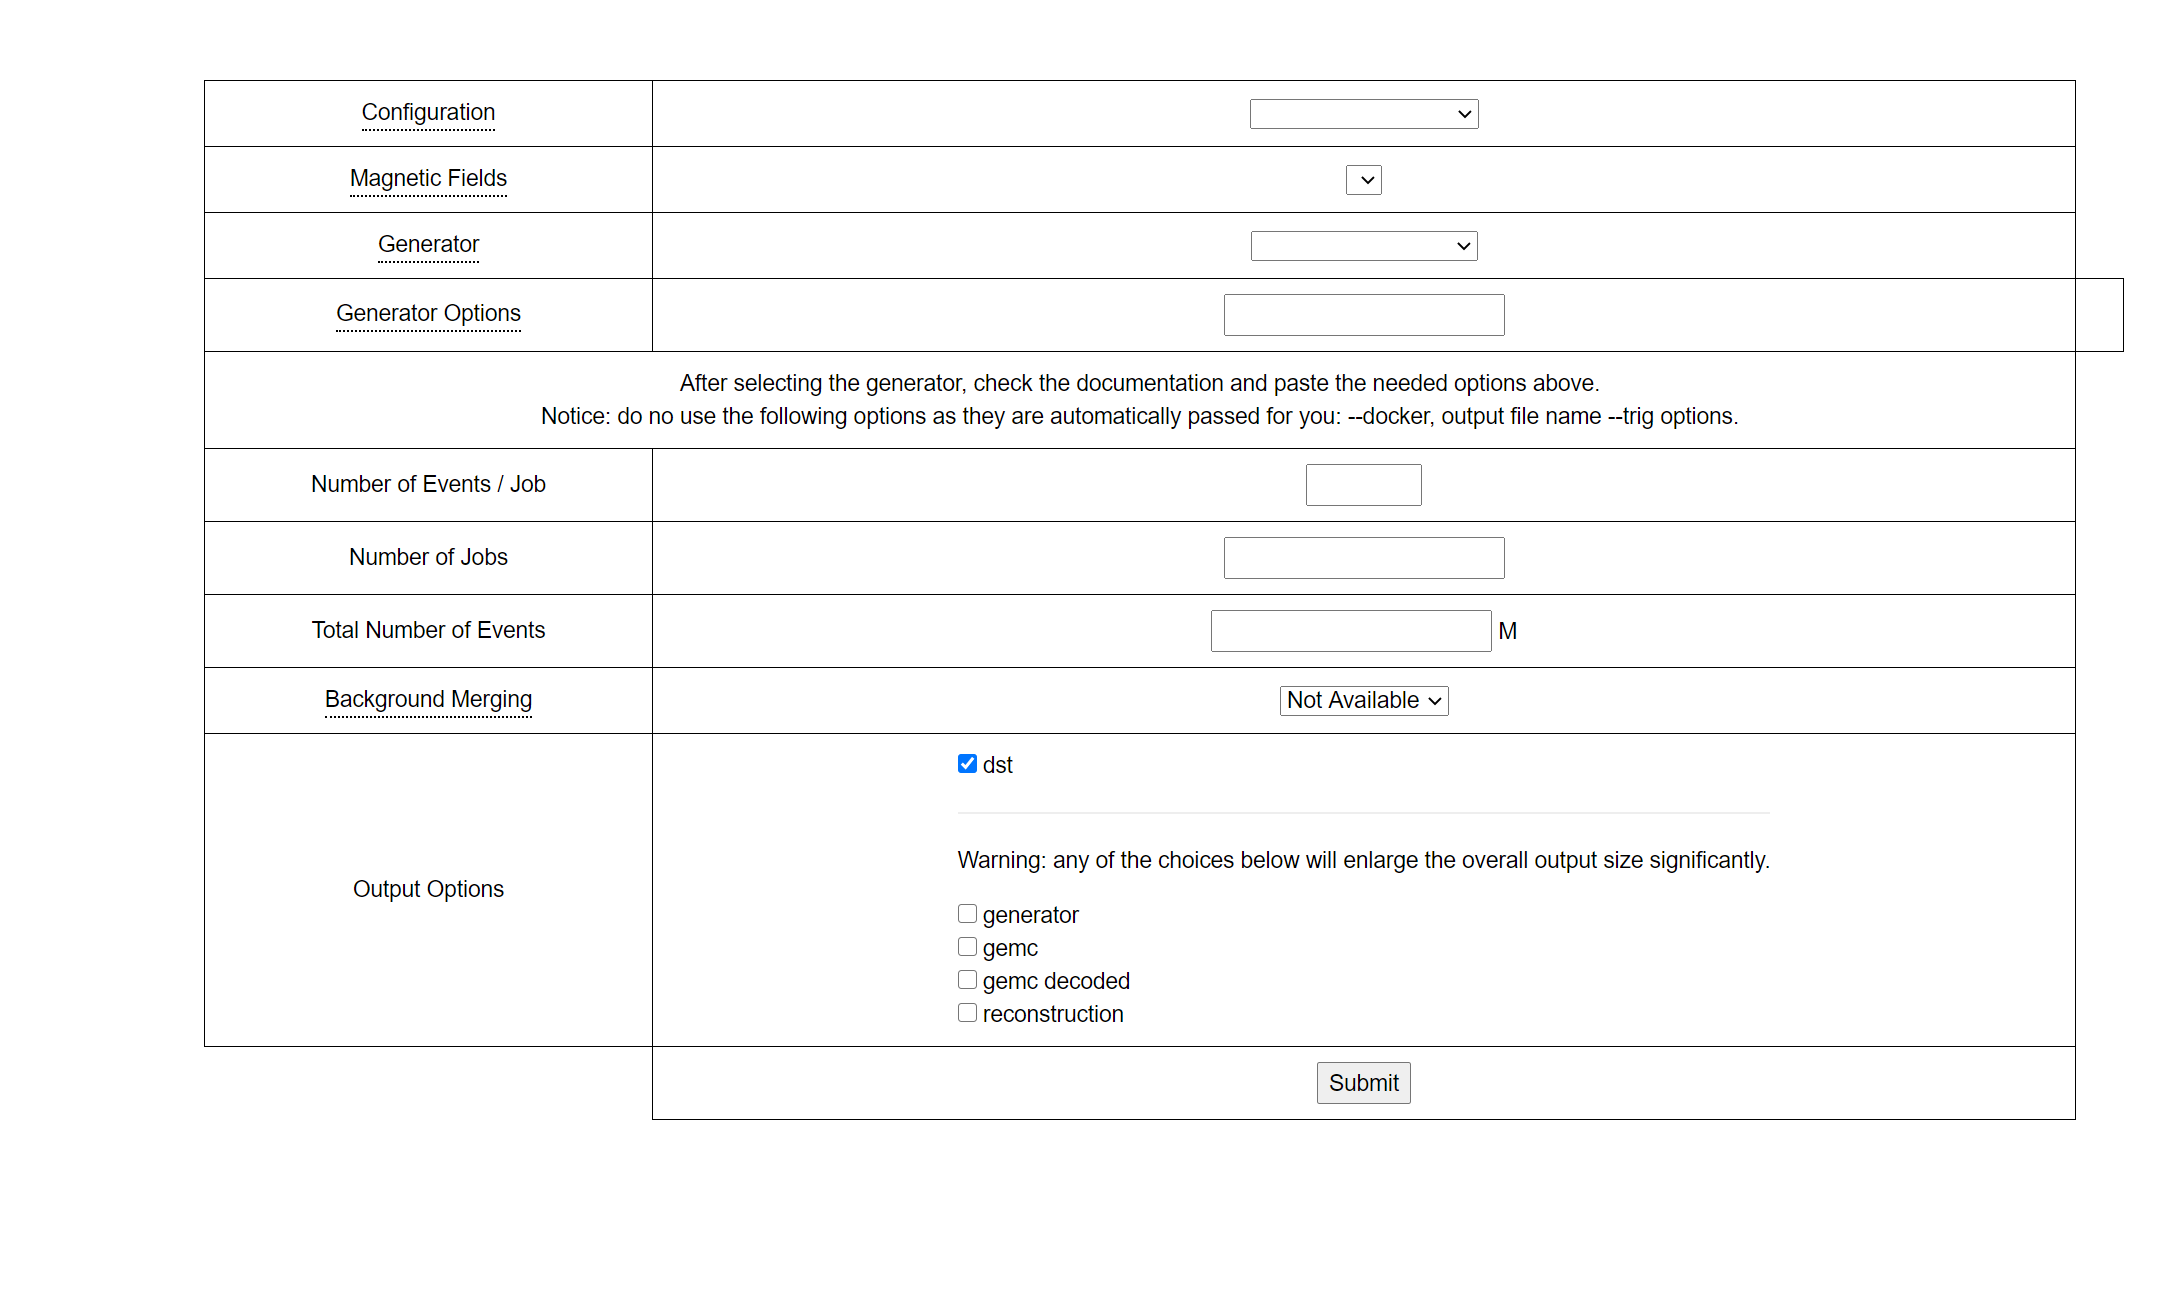
\includegraphics[width=16cm]{xxTasks/pics/pullthisin.png}
        \end{figure}


\section{Future Improvements}
    List of improvememnts that are not critical but might be nice in the future for someone who has time. Also these might be pushed up to more critical at any given time.
    \subsection{Include Priority}
        add priority to JSON (not to be used on normal production page, just the test page)
       SubMit/utils/update\_priority.py
    
       This is the way we handle priority P , which is basically P =  (constant) / N Running Jobs
    
    \subsection{Email Monitoring}
        If someone has the time, it is straightforward to set up triggers in python to send emails if things are broken. This would help in the case of system breaks. But, simulations do not usually run on ultra-critical time schedueles, so this is less important.
    \subsection{Live Generation and Usage of Container and Experiments}
        Generate in live-time on the webportal dependent quantities such as generator lists, configuration files, background merging file list 
    \subsection{Dynamic GCard Descriptions}
        Set up a dynamic list of gcards acceptable have list returned to user on what gcards are valid, can assume clas12.gcard \& a description of what gcard is / does / has in it
        Regarding the gcards, I think it's ok to have them in a file for now. We can wait a few container releases to see if what's in the file matches the container content or it has to be different. 
        The command to retrieve the list from the container is straightforward:
        
        \begin{lstlisting}
            singularity exec --home ${PWD}:/srv --pwd /srv --bind /cvmfs --contain --ipc --pid /cvmfs/singularity.opensciencegrid.org/jeffersonlab/clas12simulations:production ls /jlab/work/ | grep gcard
        \end{lstlisting}
        
    \subsection{Better Metrics / Logging}
        How will we log the number of events / the number of jobs if the user supplies the gcards / LUND files?
        use log output files to monitor job submissions



\end{document}
